
\subsection{Real time communications}\label{rtc}

\ac{WebRTC} is an open source technology that defines a collection of standard protocols and JavaScript \ac{API}s for web browser based real time communications without installing any additional application or plug-in. 

Some operating systems such as \emph{Android}, \emph{iOS}, \emph{Linux}, \emph{OSX} and \emph{Windows} implement native \ac{WebRTC} libraries, extending the usage of \ac{WebRTC} to applications outside the web browser. This native support can help to implement applications that record video and audio streams for further playback.

%RP indicar que agora também já temos webrtc fora do browser devido ao seu sucesso e ao facto de reunir tecnologia state of the art?

\begin{figure}[H]
	\centering
	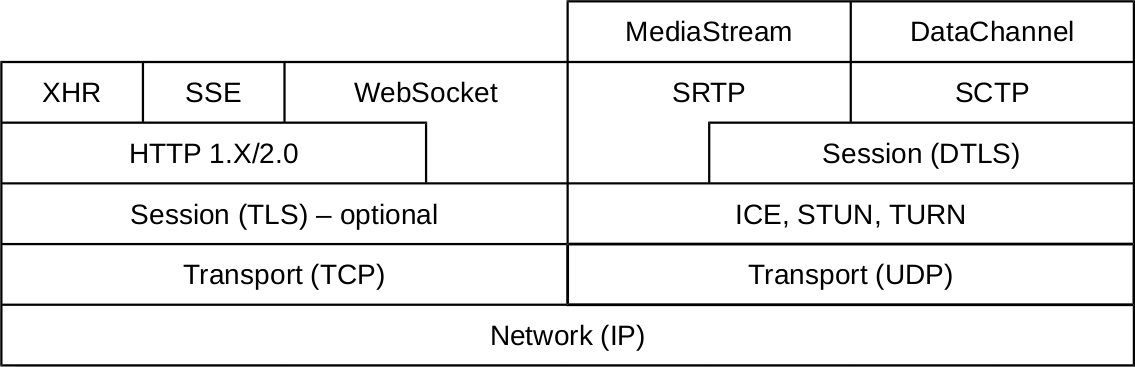
\includegraphics[width=0.8\textwidth]{figures/webrtc_stack.png}
	\caption{WebRTC protocol Stack}
\end{figure}

\ac{WebRTC} defines three main \ac{API}s: MediaStream, PeerConnection and DataChannel. 

\begin{itemize}
  \item \textbf{MediaStream} allows the browser to access the camera, microphone and the device's screen. 

  \item \textbf{PeerConnection} acquires connection data and negotiates with peers.
%RP establishes and negociates a connection with a peer for transmitting real-time video or audio?
  \item \textbf{DataChannel} provides a channel for exchanging arbitrary data with other peers.
\end{itemize}

\ac{WebRTC} uses \ac{UDP} for transporting data, which provides lower latencies than \ac{TCP}, but is not reliable and does not assure packet order and integrity. \ac{SCTP} and \ac{SRTP} are used for streaming data, providing a mechanism for congestion control and partial reliable delivery over \ac{UDP}. All transferred audio, data and video must be encrypted with \ac{DTLS} symmetric keys. \ac{DTLS} provides the same security guarantees as \ac{TLS}. 

\ac{TLS} doesn't support independent packet decryption\cite{rfc6347}, for that it requires a reliable transport channel, typically \ac{TCP}. The decryption of a packet depends on the previous packet, which for unreliable transport protocols like \ac{UDP} may represent a problem, either due to packet loss or different reception order.

\ac{DTLS} is similar to \ac{TLS}, but is used on top of \ac{UDP}.
The main difference is the inclusion of a sequence number per packet that is used for packet re-ordering on reception and protects from duplicated packets. If a packet sequence number is less than the expected sequence number the packet is discarded. If a packet sequence number is greater than the expected sequence number the packet may be enqueued or discarded. By knowing the sequence of messages that are sent and received in \ac{DTLS}, timers are used for packet retransmission avoiding acknowledgment messages.
%RP TLS?

\begin{figure}[H]
	\centering
	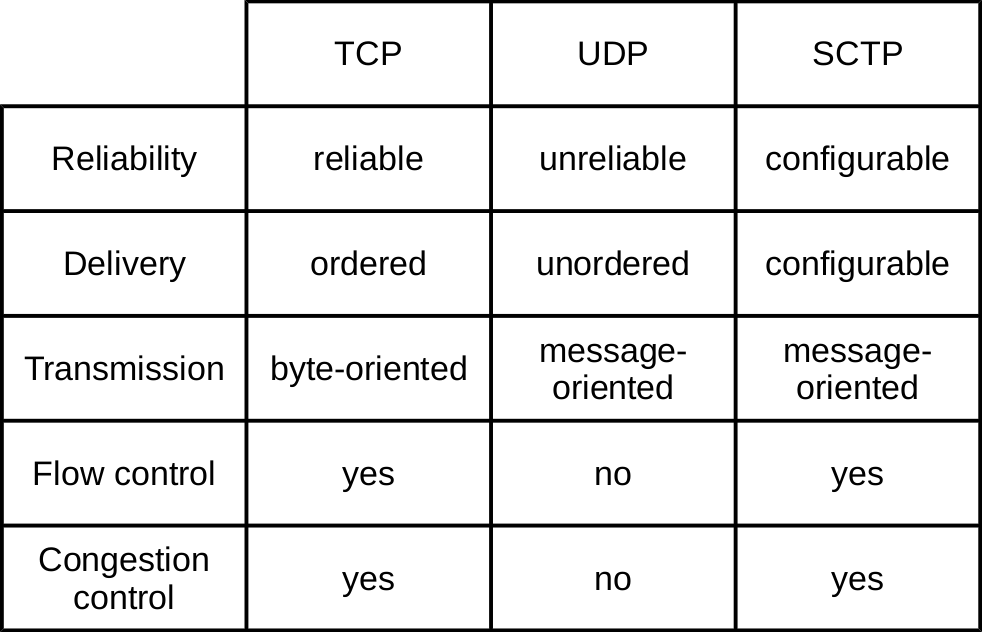
\includegraphics[width=0.6\textwidth]{figures/basic_protocols.png}
	\caption{Overview of transport protocols}
\end{figure}

\ac{WebRTC}'s \emph{DataChannel} is built on top of \ac{SCTP}, which is encapsulated by \ac{DTLS}. \ac{DTLS} encapsulation provides confidentiality, authentication and integrity to the transfered data. A \emph{Data Channel} has one incoming stream and one outgoing stream, providing bidirectional communication. Each data channel direction can be configured for reliable or unreliable transmission, the same can be done for order delivery and priority. which can also be defined for improving the quality of service of a particular stream over the others.

\ac{WebRTC}'s \emph{MediaStream} is built on top of \ac{SRTP}, which requires an external mechanism for key exchange. \ac{DTLS} keys are negotiated on handshake in order to achieve a secure connection. The new keys derived from \ac{DTLS} handshake are seized for \ac{SRTP} encryption, the remaining \ac{SRTP} communications are done through \ac{UDP} without using \ac{DTLS}.
%RP quais remaining?  A última frase é confusa

\ac{WebRTC} aims to provide a standard platform for real-time audio and video on the Web. It arrives at a time when several proprietary products are well established.
\emph{Skype}\footnote{\url{http://www.skype.com/}(accessed June 1, 2015).} is an application that allows video, voice, instant messaging and multi-party communication over proprietary protocols, its main strength are the amount of users that are using it nowadays and the ability to perform voice calls to the \ac{PSTN}. But compared to \emph{Skype}, \ac{WebRTC} applications don't need to be pre-installed.

\emph{Google Hangouts}\footnote{\url{http://plus.google.com/hangouts}(accessed June 1, 2015).} is another popular video multi-party conference web application. 
In the past, in order to use \emph{hangouts} on a web browser a plug-in had to be installed, nowadays hangouts is using \ac{WebRTC}. \emph{Google Hangouts} supports viewing videos on \emph{youtube} synchronously, drawing collaboratively, creating music and playing multi-player games. These applications are implemented with \emph{Adobe Flash}.  

\emph{Jitsi Meet}\footnote{\url{http://jitsi.org/Projects/JitsiMeet}(accessed June 1, 2015).} is a \ac{WebRTC} collaborative application that uses \emph{Jitsi Videobridge} for high quality and scalable video conferences and supports shared document editing. \emph{Jitsi Meet} allows a great amount of users in the same conversation by identifying the current most active participant users and, by consequence, reducing the video and audio quality for all the other users. \emph{Jitsi Videobridge} is a server that enables multi-party video calls. 

%RP a descricção do skype, hangouts e jistsi cai um pouco do céu. Não há uma transição e não é feita uma análise. Apenas são indicados. Não há comparação entre eles nem com o que pode ser feito por webrtc.


